\chapter{LLMalMorph 的详细设计}

\section{A. LLMalMorph 框架}

在本节中,我们将详细阐述我们框架的架构(见图\ref{fig:4.1})。LLMalMorph 分为两个主要模块。第一个模块功能变异模块使用 LLM 和策略性生成的提示来转换恶意软件源代码函数。第二个模块 变种合成模块将转换后的函数集成回源代码,编译修改后的项目以生成恶意软件变体。该模块还融入了人在回路流程用于编译期间的调试。第一个模块又包含三个关键子模块:Extractor、Prompt Generator 和 LLM Based Function Modifier。第二个模块包含两个主要子模块:Merger 以及 Compilation and Debugging。我们现在介绍支撑该框架的形式化算法,随后对各模块进行详细解释。

\begin{figure}[htbp]
	\centering
	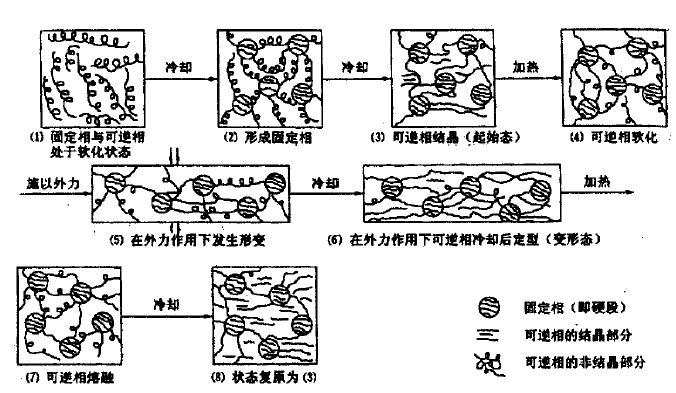
\includegraphics[width=0.75\textwidth]{figures/figure1.png}
	% \caption[这里的文字将会显示在 listoffigure 中]{这里的文字将会显示在正文中}
	\caption{LLMalMorph整体架构。该框架由两大核心模块构成:功能变异模块:从恶意软件源代码文件中提取功能函数,并借助LLM进行修改。变种合成模块:将修改后的函数更新至恶意软件源代码,通过编译项目生成变种文件}\label{fig:4.1}
\end{figure}

Algorithm 1,专为功能变异模块设计,详细说明了三个子模块 Extractor、Prompt Generator 和 LLM-Based Function Modifier 如何转换恶意软件源代码中的函数。该算法以文件名 $i$、要修改的函数数量 $j$、期望的转换策略 $s$ 以及选定的 $LLM$ 作为输入。接下来,我们将详细描述每个子模块。

\begin{algorithm}[htbp]
	\caption{使用LLM转换函数}
	\KwIn{文件名$i$,需要改变的函数数量 $j$,转换策略 $s$,语言模型 $LLM$}
	\KwOut{转换后的函数集$\hat{F_{s}}=\{\hat{f_{1}^{i}},\hat{f_{2}^{i}}...,\hat{f_{j}^{i}}\}$}

    Headers,globals,functions$\{f_{1}^{i},f_{2}^{i},...,f_{G}^{i}\}\leftarrow extractor(i)$;
    Initialize transformed function set $\hat{F_{s}}\leftarrow \emptyset$;

    \For{$t \gets 1$ \KwTo $j$}{
        $p_{s}||f_{t}^{i} \leftarrow gen_prompt(s,f_{t}^{i},headers,globals)$;\\
        Transform function: $\hat{f_{t}^{i}} \leftarrow LLM(p_{s}||f_{t}^{i})$;\\
        Update set: $\hat{F_{s}} \leftarrow \hat{F_{s}} \cup \{\hat{f_{t}^{i}}\}$;
    }
    return $\hat{F_{s}}$
\end{algorithm}